\documentclass[]{book}
\usepackage{lmodern}
\usepackage{amssymb,amsmath}
\usepackage{ifxetex,ifluatex}
\usepackage{fixltx2e} % provides \textsubscript
\ifnum 0\ifxetex 1\fi\ifluatex 1\fi=0 % if pdftex
  \usepackage[T1]{fontenc}
  \usepackage[utf8]{inputenc}
\else % if luatex or xelatex
  \ifxetex
    \usepackage{mathspec}
  \else
    \usepackage{fontspec}
  \fi
  \defaultfontfeatures{Ligatures=TeX,Scale=MatchLowercase}
\fi
% use upquote if available, for straight quotes in verbatim environments
\IfFileExists{upquote.sty}{\usepackage{upquote}}{}
% use microtype if available
\IfFileExists{microtype.sty}{%
\usepackage{microtype}
\UseMicrotypeSet[protrusion]{basicmath} % disable protrusion for tt fonts
}{}
\usepackage{hyperref}
\hypersetup{unicode=true,
            pdftitle={Uso do sistema R para análise de dados},
            pdfauthor={Jefferson Vieira José, André Pereira Freire Ferraz},
            pdfborder={0 0 0},
            breaklinks=true}
\urlstyle{same}  % don't use monospace font for urls
\usepackage{natbib}
\bibliographystyle{apalike}
\usepackage{color}
\usepackage{fancyvrb}
\newcommand{\VerbBar}{|}
\newcommand{\VERB}{\Verb[commandchars=\\\{\}]}
\DefineVerbatimEnvironment{Highlighting}{Verbatim}{commandchars=\\\{\}}
% Add ',fontsize=\small' for more characters per line
\usepackage{framed}
\definecolor{shadecolor}{RGB}{248,248,248}
\newenvironment{Shaded}{\begin{snugshade}}{\end{snugshade}}
\newcommand{\AlertTok}[1]{\textcolor[rgb]{0.94,0.16,0.16}{#1}}
\newcommand{\AnnotationTok}[1]{\textcolor[rgb]{0.56,0.35,0.01}{\textbf{\textit{#1}}}}
\newcommand{\AttributeTok}[1]{\textcolor[rgb]{0.77,0.63,0.00}{#1}}
\newcommand{\BaseNTok}[1]{\textcolor[rgb]{0.00,0.00,0.81}{#1}}
\newcommand{\BuiltInTok}[1]{#1}
\newcommand{\CharTok}[1]{\textcolor[rgb]{0.31,0.60,0.02}{#1}}
\newcommand{\CommentTok}[1]{\textcolor[rgb]{0.56,0.35,0.01}{\textit{#1}}}
\newcommand{\CommentVarTok}[1]{\textcolor[rgb]{0.56,0.35,0.01}{\textbf{\textit{#1}}}}
\newcommand{\ConstantTok}[1]{\textcolor[rgb]{0.00,0.00,0.00}{#1}}
\newcommand{\ControlFlowTok}[1]{\textcolor[rgb]{0.13,0.29,0.53}{\textbf{#1}}}
\newcommand{\DataTypeTok}[1]{\textcolor[rgb]{0.13,0.29,0.53}{#1}}
\newcommand{\DecValTok}[1]{\textcolor[rgb]{0.00,0.00,0.81}{#1}}
\newcommand{\DocumentationTok}[1]{\textcolor[rgb]{0.56,0.35,0.01}{\textbf{\textit{#1}}}}
\newcommand{\ErrorTok}[1]{\textcolor[rgb]{0.64,0.00,0.00}{\textbf{#1}}}
\newcommand{\ExtensionTok}[1]{#1}
\newcommand{\FloatTok}[1]{\textcolor[rgb]{0.00,0.00,0.81}{#1}}
\newcommand{\FunctionTok}[1]{\textcolor[rgb]{0.00,0.00,0.00}{#1}}
\newcommand{\ImportTok}[1]{#1}
\newcommand{\InformationTok}[1]{\textcolor[rgb]{0.56,0.35,0.01}{\textbf{\textit{#1}}}}
\newcommand{\KeywordTok}[1]{\textcolor[rgb]{0.13,0.29,0.53}{\textbf{#1}}}
\newcommand{\NormalTok}[1]{#1}
\newcommand{\OperatorTok}[1]{\textcolor[rgb]{0.81,0.36,0.00}{\textbf{#1}}}
\newcommand{\OtherTok}[1]{\textcolor[rgb]{0.56,0.35,0.01}{#1}}
\newcommand{\PreprocessorTok}[1]{\textcolor[rgb]{0.56,0.35,0.01}{\textit{#1}}}
\newcommand{\RegionMarkerTok}[1]{#1}
\newcommand{\SpecialCharTok}[1]{\textcolor[rgb]{0.00,0.00,0.00}{#1}}
\newcommand{\SpecialStringTok}[1]{\textcolor[rgb]{0.31,0.60,0.02}{#1}}
\newcommand{\StringTok}[1]{\textcolor[rgb]{0.31,0.60,0.02}{#1}}
\newcommand{\VariableTok}[1]{\textcolor[rgb]{0.00,0.00,0.00}{#1}}
\newcommand{\VerbatimStringTok}[1]{\textcolor[rgb]{0.31,0.60,0.02}{#1}}
\newcommand{\WarningTok}[1]{\textcolor[rgb]{0.56,0.35,0.01}{\textbf{\textit{#1}}}}
\usepackage{longtable,booktabs}
\usepackage{graphicx,grffile}
\makeatletter
\def\maxwidth{\ifdim\Gin@nat@width>\linewidth\linewidth\else\Gin@nat@width\fi}
\def\maxheight{\ifdim\Gin@nat@height>\textheight\textheight\else\Gin@nat@height\fi}
\makeatother
% Scale images if necessary, so that they will not overflow the page
% margins by default, and it is still possible to overwrite the defaults
% using explicit options in \includegraphics[width, height, ...]{}
\setkeys{Gin}{width=\maxwidth,height=\maxheight,keepaspectratio}
\IfFileExists{parskip.sty}{%
\usepackage{parskip}
}{% else
\setlength{\parindent}{0pt}
\setlength{\parskip}{6pt plus 2pt minus 1pt}
}
\setlength{\emergencystretch}{3em}  % prevent overfull lines
\providecommand{\tightlist}{%
  \setlength{\itemsep}{0pt}\setlength{\parskip}{0pt}}
\setcounter{secnumdepth}{5}
% Redefines (sub)paragraphs to behave more like sections
\ifx\paragraph\undefined\else
\let\oldparagraph\paragraph
\renewcommand{\paragraph}[1]{\oldparagraph{#1}\mbox{}}
\fi
\ifx\subparagraph\undefined\else
\let\oldsubparagraph\subparagraph
\renewcommand{\subparagraph}[1]{\oldsubparagraph{#1}\mbox{}}
\fi

%%% Use protect on footnotes to avoid problems with footnotes in titles
\let\rmarkdownfootnote\footnote%
\def\footnote{\protect\rmarkdownfootnote}

%%% Change title format to be more compact
\usepackage{titling}

% Create subtitle command for use in maketitle
\providecommand{\subtitle}[1]{
  \posttitle{
    \begin{center}\large#1\end{center}
    }
}

\setlength{\droptitle}{-2em}

  \title{Uso do sistema R para análise de dados}
    \pretitle{\vspace{\droptitle}\centering\huge}
  \posttitle{\par}
    \author{Jefferson Vieira José, André Pereira Freire Ferraz}
    \preauthor{\centering\large\emph}
  \postauthor{\par}
      \predate{\centering\large\emph}
  \postdate{\par}
    \date{2019-08-01}

\usepackage{booktabs}

\begin{document}
\maketitle

{
\setcounter{tocdepth}{1}
\tableofcontents
}
\hypertarget{pre-requisitos}{%
\chapter{Pré requisitos}\label{pre-requisitos}}

Material em construção.

\hypertarget{intro}{%
\chapter{R Básico}\label{intro}}

Iremos abordar as expressões básicas do R.
Começaremos simples, com \textbf{números}, \textbf{strings} e valores \textbf{true/false}. Em seguida, mostraremos como armazenar esses valores em variáveis e como transmiti-los as funções. Como obter ajuda sobre as funções e no final vamos carregar um arquivo

\hypertarget{expressoes}{%
\section{Expressões}\label{expressoes}}

Digite seu nome no prompt, e o R irá avalio-lo e imprimir a resposta.
Vamos tentar matemática simples. Digite o comando abaixo e aperte enter

\begin{Shaded}
\begin{Highlighting}[]
\DecValTok{2}\OperatorTok{+}\DecValTok{8}
\end{Highlighting}
\end{Shaded}

\begin{verbatim}
## [1] 10
\end{verbatim}

Note que é impresso o resultado, 10.
Digite a frase ``Engenharia Agrícola''

\begin{Shaded}
\begin{Highlighting}[]
\StringTok{"Engenharia Agrícola"}
\end{Highlighting}
\end{Shaded}

\begin{verbatim}
## [1] "Engenharia Agrícola"
\end{verbatim}

Agora tente multiplicar 6 vezes 5 (* é o operador de multiplicação).

\begin{Shaded}
\begin{Highlighting}[]
\DecValTok{6}\OperatorTok{*}\DecValTok{5}
\end{Highlighting}
\end{Shaded}

\begin{verbatim}
## [1] 30
\end{verbatim}

\hypertarget{valores-truefalso}{%
\section{Valores true/falso}\label{valores-truefalso}}

Algumas expressões retornam um ``valor lógico'': TRUE ou FALSE e/ou ``booleanos''.
Vamos tentar digitar uma expressões que nos dá um valor lógico:

\begin{Shaded}
\begin{Highlighting}[]
\DecValTok{7}\OperatorTok{<}\DecValTok{12}
\end{Highlighting}
\end{Shaded}

\begin{verbatim}
## [1] TRUE
\end{verbatim}

E outro valor lógico (sinal duplo de igualdade)

\begin{Shaded}
\begin{Highlighting}[]
\DecValTok{6}\OperatorTok{+}\DecValTok{5}\OperatorTok{==}\DecValTok{10}
\end{Highlighting}
\end{Shaded}

\begin{verbatim}
## [1] FALSE
\end{verbatim}

\textbf{T} e \textbf{F} são taquigrafia para TRUE e FALSE. Tente isso:

\begin{Shaded}
\begin{Highlighting}[]
\NormalTok{F}\OperatorTok{==}\OtherTok{FALSE}
\end{Highlighting}
\end{Shaded}

\begin{verbatim}
## [1] TRUE
\end{verbatim}

\hypertarget{variaveis}{%
\section{Variáveis}\label{variaveis}}

Você pode armazenar valores em uma variável para usar mais tarde.
Digite \textbf{x \textless{}- 28} para armazenar um valor em \textbf{x}.

\begin{Shaded}
\begin{Highlighting}[]
\NormalTok{x<-}\DecValTok{28}
\end{Highlighting}
\end{Shaded}

Tende dividr \textbf{x} por \textbf{4}( \textbf{/} é o operador da divisão).

\begin{Shaded}
\begin{Highlighting}[]
\NormalTok{x}\OperatorTok{/}\DecValTok{4}
\end{Highlighting}
\end{Shaded}

\begin{verbatim}
## [1] 7
\end{verbatim}

Você pode retribuir qualquer valor a uma variável a qualquer momento.
Tente atribuir ``Engenharia Agrícola''em x.

\begin{Shaded}
\begin{Highlighting}[]
\NormalTok{x <-}\StringTok{ "Engenharia Agrícola"}
\end{Highlighting}
\end{Shaded}

Tente imprimir o valor atual de x.

\begin{Shaded}
\begin{Highlighting}[]
\NormalTok{x}
\end{Highlighting}
\end{Shaded}

\begin{verbatim}
## [1] "Engenharia Agrícola"
\end{verbatim}

\hypertarget{funcoes}{%
\section{Funções}\label{funcoes}}

Você pode chamar uma \textbf{função} digitando seu nome, seguido de um ou mais argumentos para essa função entre parênteses.

Vamos tentar usar a função \textbf{sum}, para adicionar alguns números. Entrar:

\begin{Shaded}
\begin{Highlighting}[]
\KeywordTok{sum}\NormalTok{ (}\DecValTok{2}\NormalTok{, }\DecValTok{4}\NormalTok{, }\DecValTok{6}\NormalTok{)}
\end{Highlighting}
\end{Shaded}

\begin{verbatim}
## [1] 12
\end{verbatim}

Alguns argumentos têm nomes. Por exemplo, para repetir um valor 3 vezes, você chamaria a função \textbf{rep} e forneceria seu argumento \textbf{times}:

\begin{Shaded}
\begin{Highlighting}[]
\KeywordTok{rep}\NormalTok{(}\StringTok{"Engenharia Agrícola"}\NormalTok{, }\DataTypeTok{times=}\DecValTok{3}\NormalTok{)}
\end{Highlighting}
\end{Shaded}

\begin{verbatim}
## [1] "Engenharia Agrícola" "Engenharia Agrícola" "Engenharia Agrícola"
\end{verbatim}

Tente chamar a função \textbf{sqrt} para obter a raiz quadrada 16.

\begin{Shaded}
\begin{Highlighting}[]
\KeywordTok{sqrt}\NormalTok{(}\DecValTok{16}\NormalTok{)}
\end{Highlighting}
\end{Shaded}

\begin{verbatim}
## [1] 4
\end{verbatim}

\hypertarget{ajuda}{%
\section{Ajuda}\label{ajuda}}

A função \textbf{help ( )} traz ajuda para a função desejada. Tente exibir ajuda para a função \textbf{mean}:

\begin{Shaded}
\begin{Highlighting}[]
\KeywordTok{help}\NormalTok{ (mean)}
\end{Highlighting}
\end{Shaded}

A função \textbf{example ( )} traz exemplos de usos. Tente exibir exemplos para a função \textbf{min}:

\begin{Shaded}
\begin{Highlighting}[]
\KeywordTok{example}\NormalTok{(min)}
\end{Highlighting}
\end{Shaded}

\begin{verbatim}
## 
## min> require(stats); require(graphics)
## 
## min>  min(5:1, pi) #-> one number
## [1] 1
## 
## min> pmin(5:1, pi) #->  5  numbers
## [1] 3.141593 3.141593 3.000000 2.000000 1.000000
## 
## min> x <- sort(rnorm(100));  cH <- 1.35
## 
## min> pmin(cH, quantile(x)) # no names
## [1] -2.35431565 -0.73721231 -0.03061528  0.76060334  1.35000000
## 
## min> pmin(quantile(x), cH) # has names
##          0%         25%         50%         75%        100% 
## -2.35431565 -0.73721231 -0.03061528  0.76060334  1.35000000 
## 
## min> plot(x, pmin(cH, pmax(-cH, x)), type = "b", main =  "Huber's function")
\end{verbatim}

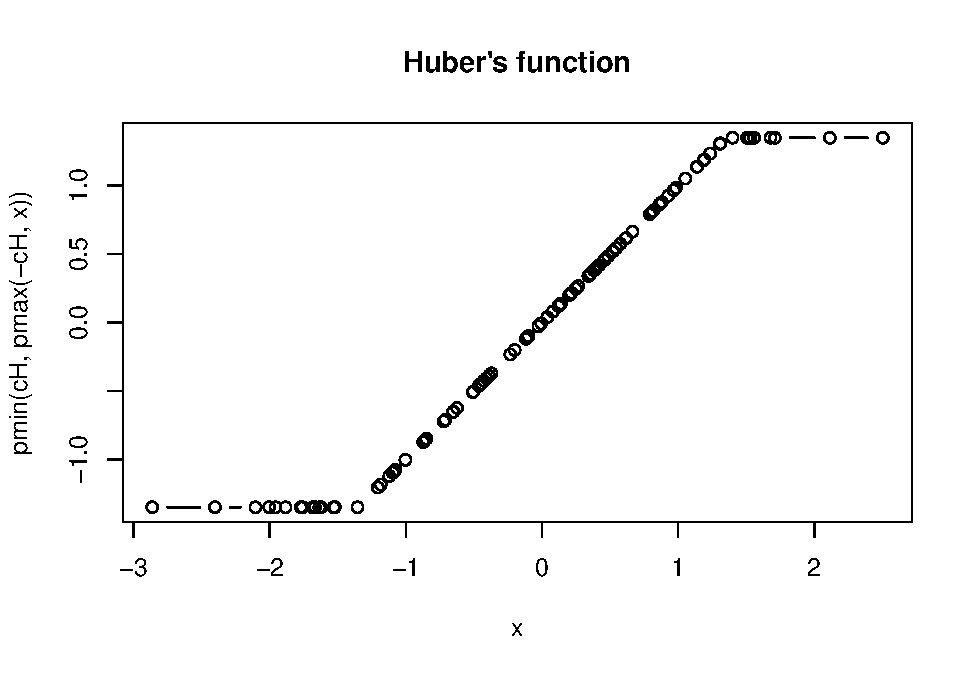
\includegraphics{TudodoR_files/figure-latex/unnamed-chunk-14-1.pdf}

\begin{verbatim}
## 
## min> cut01 <- function(x) pmax(pmin(x, 1), 0)
## 
## min> curve(      x^2 - 1/4, -1.4, 1.5, col = 2)
\end{verbatim}

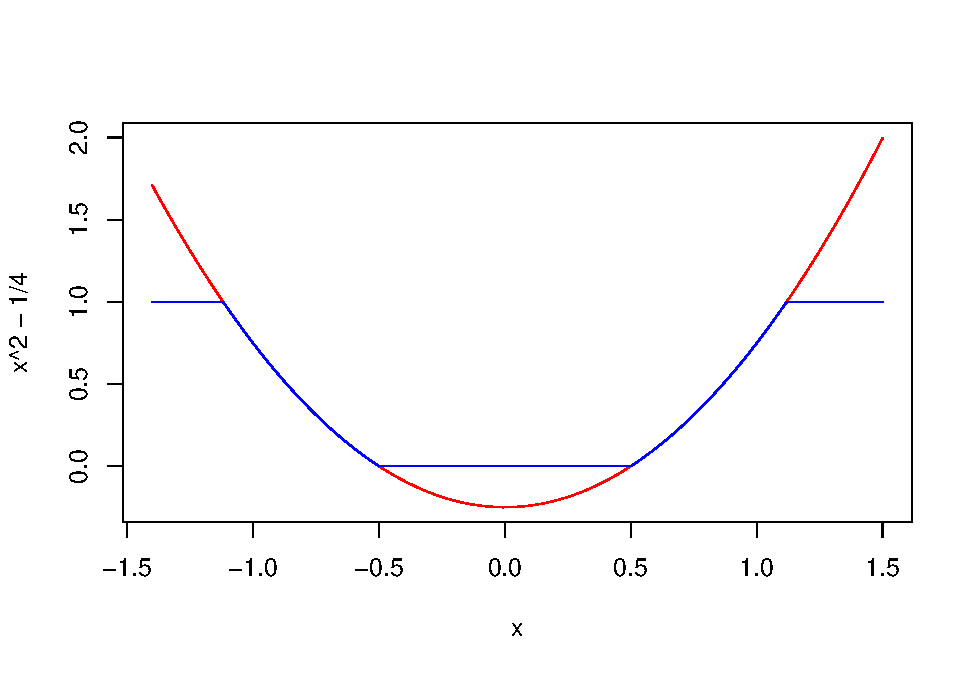
\includegraphics{TudodoR_files/figure-latex/unnamed-chunk-14-2.pdf}

\begin{verbatim}
## 
## min> curve(cut01(x^2 - 1/4), col = "blue", add = TRUE, n = 500)
## 
## min> ## pmax(), pmin() preserve attributes of *first* argument
## min> D <- diag(x = (3:1)/4) ; n0 <- numeric()
## 
## min> stopifnot(identical(D,  cut01(D) ),
## min+           identical(n0, cut01(n0)),
## min+           identical(n0, cut01(NULL)),
## min+           identical(n0, pmax(3:1, n0, 2)),
## min+           identical(n0, pmax(n0, 4)))
\end{verbatim}

\hypertarget{referencia}{%
\section{Referência}\label{referencia}}

MELO, M. P.; PETERNELI, L. A. \textbf{Conhecendo o R: Um visão mais que estatística}. Viçosa, MG: UFV, 2013. 222p.

\textbf{Prof.~Paulo Justiniando Ribeiro} \textgreater{}\url{http://www.leg.ufpr.br/~paulojus/}\textless{}

\textbf{Prof.~Adriano Azevedo Filho} \textgreater{}\url{http://rpubs.com/adriano/esalq2012inicial}\textless{}

\textbf{Prof.~Fernando de Pol Mayer} \textgreater{}\url{https://fernandomayer.github.io/ce083-2016-2/}\textless{}

\textbf{Site Interativo Datacamp} \textgreater{}\url{https://www.datacamp.com/}\textless{}

\hypertarget{literature}{%
\chapter{Literature}\label{literature}}

Here is a review of existing methods.

\hypertarget{methods}{%
\chapter{Methods}\label{methods}}

We describe our methods in this chapter.

\hypertarget{applications}{%
\chapter{Applications}\label{applications}}

Some \emph{significant} applications are demonstrated in this chapter.

\hypertarget{example-one}{%
\section{Example one}\label{example-one}}

\hypertarget{example-two}{%
\section{Example two}\label{example-two}}

\hypertarget{final-words}{%
\chapter{Final Words}\label{final-words}}

We have finished a nice book.

\bibliography{book.bib,packages.bib}


\end{document}
